\date{} 
\usepackage{usenix} 
\title{
\Large 
\bf Reducing Data Center Latency
}

for single author \author{ 
{\rm Zainab Ghadiyali}\\ Department of Computer
Science, University of Wisconsin-Madison 
\and {\rm Michael Griepentrog}\\
Department of Computer Science, University of Wisconsin-Madison 
\and{\rm Aditya Akella}\\
Department of Computer Science, University of Wisconsin-Madison
} 
% end author


\maketitle

\thispagestyle{empty}


\subsection*{Abstract}

\section{Introduction} 
In the last few decades, the key focus of the network
community has been on improving the overall goodput of networks. The initial
focus on circuit switching moved to packet switching due to bandwidth and
hardware inefficiences in working with network resources for
bursty communication traffic. The Transmission Control Protocol(TCP) was
invented to address the issue of bandwidth/congestion collapse in the network
and ensure bandwidth fairness.~\cite{DCTCP,Queueing,TCP_Pacing} However network
latency has been given less importance. Most applications are throughput
oriented (e.g. email) and hence not sensitive of delivery time. Latency for
latency sensitive applications is seen as an acceptable trade-off in order to
maintain high bandwidth utilization.   
However, there is now an increasing interest in reducing latency in
datacenters. A substantial amount of computing is now shifting to data centers
and reducing latency is now easier given the confines of a building rather than
tackling the issue for the internet at large. Furthermore, ultra low latency
 sensitive applications such as High Frequency Trading, HPC and Google Instant 
Search service could especially benefit from this.
Several high-frequency traders implement trading applications with a goal to reach a
trade decision in under 100 microseconds. 
Network Interface Cards (NIC), end-host stacks and switches are all points 
where a packet may experience latency while traversing from client to server. 
In order to address delays arising from queueing delay at switches, 
DCTCP ~\cite{DCTCP} uses ECN marking to slow down flows before the queue is 
saturated. HULL ~\cite{HULL} further suggests trading off a little bandwidth to 
provide smaller amount of latency.  
In this paper, we look into understanding how switch, various offloading
parameters and hardware influences latency.

OUR OBSERVATION IS THAT

THROUGH OUR EVALUATION WE FIND THAT

\section{Methodology}
\subsection{Design}
A strong evaluation and understanding of reducing latency will be incomplete
without simulateneously studying the tradeoffs between latency and other
important factors such as bandwidth and CPU utilization. Thus, we study latency
along with its influence on CPU utilization and bandwidth. Furthermore, it would be 
important to also understand the role of latency influencing factors in UDP and
TCP. UDP should be faster than TCP since it allows a continuous packet stream
versus TCP that sends acknowledgements (ACKS) for a set of packets calculated
using the TCP window size and round trip time (RTT) Thus, metrics were obtained
for TCP and UDP flows.  Offloading moves the IP and TCP processing to the
Network Interface (NIC).  Keeping type of NIC constant, we can study the
influence of offloading on latency. TCP segmentation offload (TSO)/ Generic
segmentation offload (GSO) are considered useful in increase outbound
throughput of high-bandwidth network connections since it reduces host CPU cycles
for protocol header processing and checksumming.Generic receiving offload (GRO)
    attempts to replicate the TSO modus operandi on the receiver-side. Effects
    of offloading is studied by:

\begin{enumerate} 
\item TSO/GSO and GRO : On 
\item TSO/GSO and GRO : Off 
\item TSO/GSO : On and GRO : Off 
\item TSO/GSO : Off and GRO : On 
\end{enumerate} 

\subsection{Experimental Setup} 
Two commodity computers connected via an OpenFlow switch ~\cite{openflow}. One
of the computers served as a client and the other as server. Eight experiments
were ran in this setting. Another eight experiments ran on the two machines in
absence of OpenFlow switch. For each experiment, throughput is recorded using
iperf, cpu utilization through pidstat, interpacket delay through tcpdump and
latency through ping. This process was automated by running bash scripts on
server and client end. Offloading parameters were varied using ethtool. Data was
analysed using wireshark and a python script that parsed results from
experiments and provided basic summary in terms of min, max, stdev and average latency, 
average throughput in terms of Mbits/sec and average percent CPU utilization.
\section{Evaluation} 
\subsection{Bandwidth} 

\subsection{Offloading} 
TSO works by moving work of breaking down large chunks of data over to the NIC.
In ~/cite{avg_bandwidth_noswitch}, the x-axis represents offloading settings
while y-axis represents bandwidth. Bandwidth is almost halved
when TSO/GSO if switched off. This suggests that throughput may be increased by
switching off offloading. Keeping GRO on in the absence of TSO/GSO did not show
an appreciable change, thus suggested that GRO plays a little to no role in
increasing bandwidth. Interestingly, the bandwidth remained fairly constant for
switch as well as client despite varying offloading parameters when flows
traversed through an OpenFlow switch. 
\begin{figure}[t]
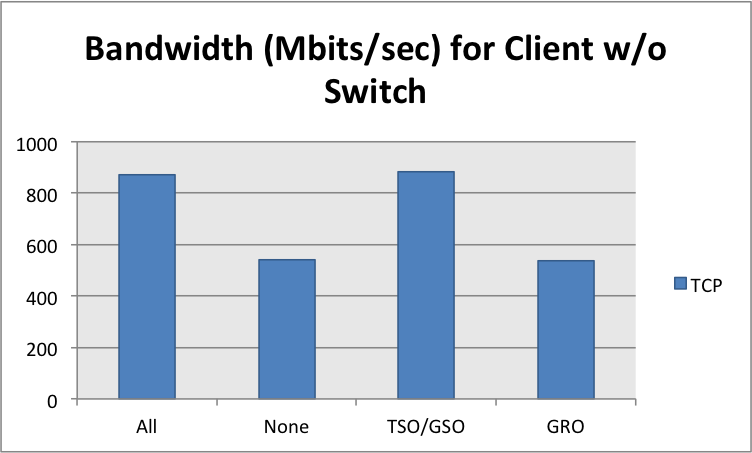
\includegraphics[scale=0.75]{avg_bandwidth_client_noswitch.png}
\caption{Bandwidth is halved when GRO or TSO/GSO/GRO is switched off}
\label{fig:avg_bandwidth_client_noswitch} \end{figure}


In ~/cite{avg_cpu_client_noswitch}, x-axis represents the offloading paramaters,
   while y-axis respresents the average percent CPU utilization for TCP and UDP
   flows for a client when flows directly traverse from client to server.
   Irrespective of offloading settings, 100\% CPU utilization is observed for
   UDP flows. This makes sense, since no offloading should occur for UDP flows.
   However, we see almost 100\% CPU utilization for TCP flows in the absence of
   TSO/GSO. This is in line with findings expressed in
   ~\cite{avg_bandwidth_client_noswitch}. Since the NIC non longer performs
   offloading, CPU is utilized for segmentation. The CPU utlization increases
   10x with a 2x decrease in bandwidth. 
\begin{figure}[t] 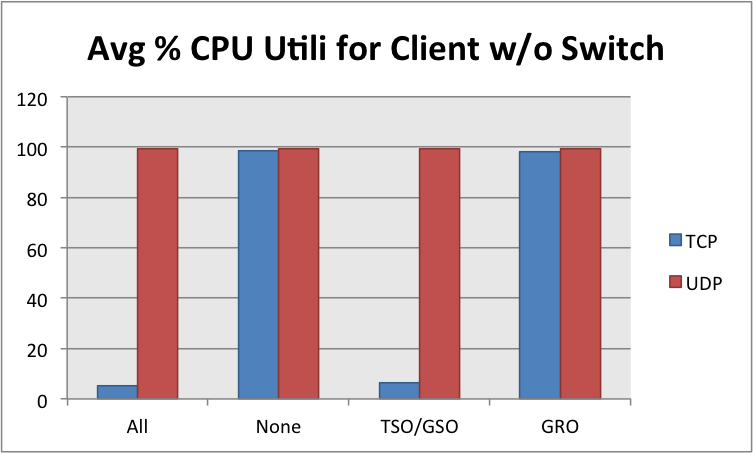
\includegraphics[scale=0.75]{avg_cpu_client_noswitch.png}
\caption{CPU utilization is maxed when GRO or TSO/GSO/GRO is switched off}
\label{fig:avg_cpu_client_noswitch} \end{figure}


\begin{figure}[t] 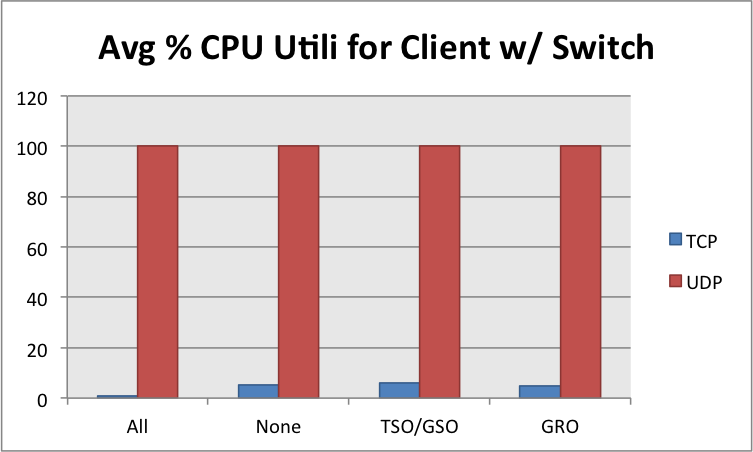
\includegraphics[scale=0.75]{avg_cpu_client_switch.png}
\caption{CPU utilization is not influenced by offloading settings in presence of
    switch} \label{fig:avg_cpu_client_switch} \end{figure}


\begin{figure}[t] 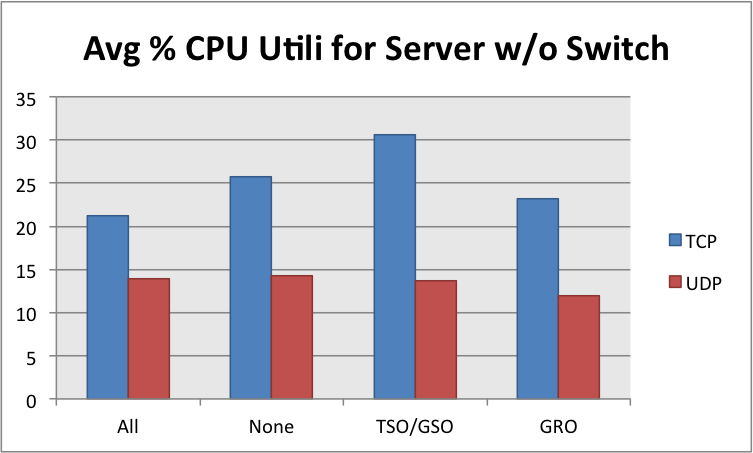
\includegraphics[scale=0.75]{avg_cpu_server_noswitch.png}
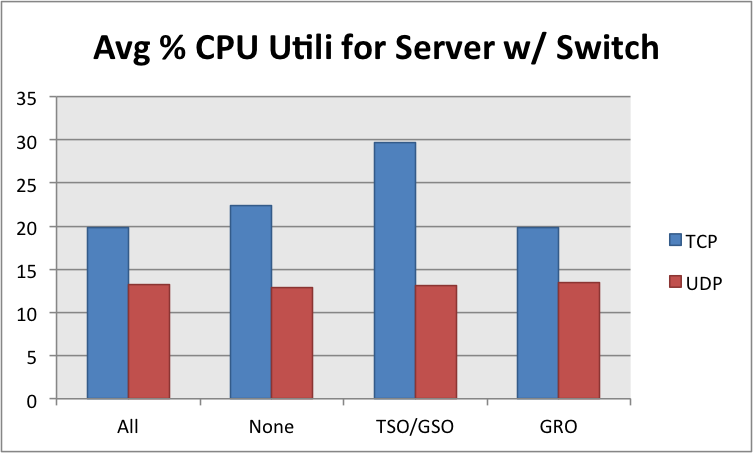
\includegraphics[scale=0.75]{avg_cpu_server_switch.png} \caption{CPU utilization
    remains fairly evenly distributed at the server end in the presence or
        absence of a switch} \label{fig:avg_cpu_server_noswitch} \end{figure}

\begin{figure}[t] \includegraphics[scale=0.75]{avg_cpu_tcp_client.png}
\caption{CPU utilization may be influenced by absence of GRO or TSP/GSO/GRO on
    the client side} \label{fig:avg_cpu_tcp_client} \end{figure}

\begin{figure}[t] 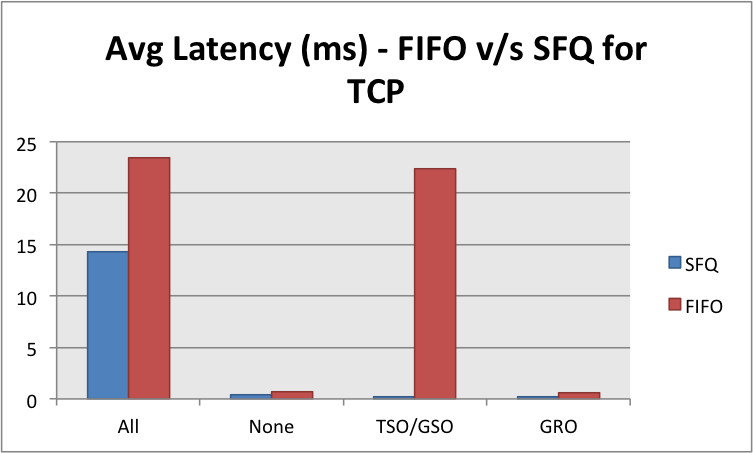
\includegraphics[scale=0.75]{avg_latency_fifo_sfq.png}
\caption{Latency remains unaffected in absence of GRO or TSO/GSO/GRO settings
    off for FIFO as well as SFQ. A significant decrease in latency is observed
        for SFQ in absence of all offloading parameters}
        \label{fig:avg_latency_fifo_sfq} \end{figure}


\begin{figure}[t] 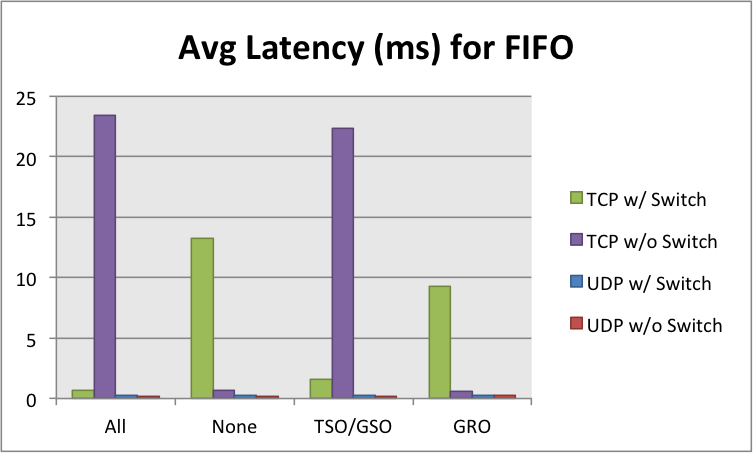
\includegraphics[scale=0.75]{avg_latency_FIFO.png}
\caption{Latency is higher for TCP thand UDP flows. Furthermore, latency is
    higher for TCP flows in absense of switch} \label{fig:avg_latency_FIFO}
    \end{figure}


\begin{figure}[t] 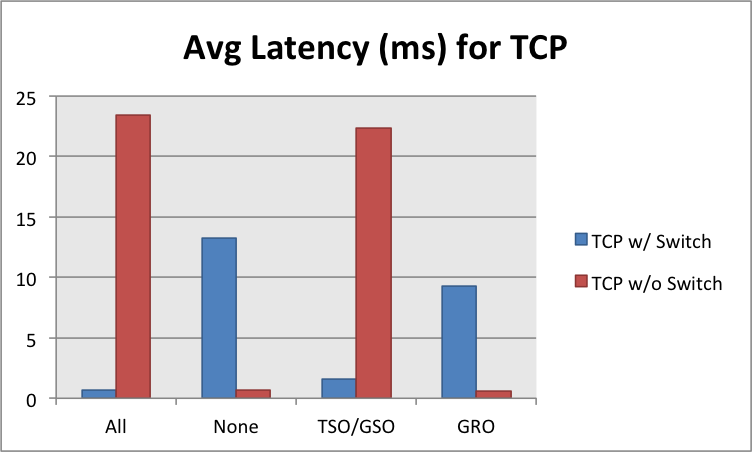
\includegraphics[scale=0.75]{avg_latency_tcp.png}
\caption{Latency is highest for TCP flows in the absense of a switch and
    presense of all or only TSO/GSO} \label{fig:avg_latency_tcp} \end{figure}


\begin{figure}[t] 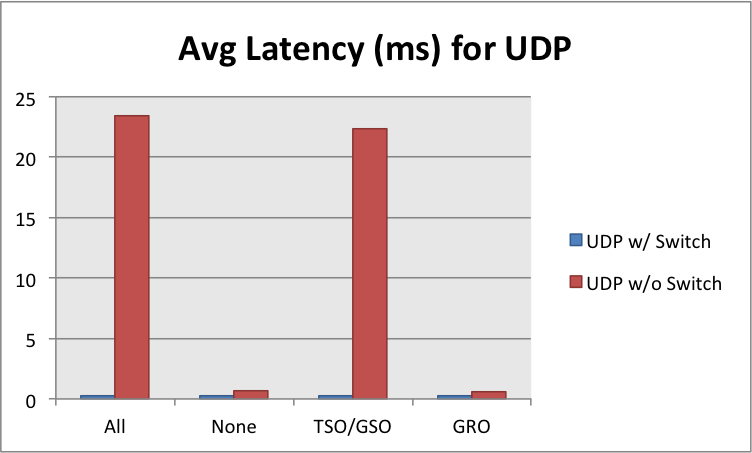
\includegraphics[scale=0.75]{avg_latency_udp.png}
\caption{Latency for UDP flows is highest in absence of a switch and presence of
    all or only TSO/GSO presnece } \label{fig:avg_latency_udp} \end{figure}

\section{Limitations and Future Work} 

\emph{Remore Direct Memory Access (RDMA)}
NICs would be interesting to study since it simplifies many problems observed
with generic TCP offloading. It would be especially interesting and important to
relate latency observed from utilizing RDMA and CPU utilization on non-RDMA
based NICs. Since RDMAs enable the network adapter to transfer data directly to
or from application memory, no work is required from CPUs, caches or context
switches.

\emph{Maximum Transmission Unit (MTU)} is the greatest amount of data that can
be transferred in one physical frame over the network. Thus, increasing MTU, may
decrease latency. The standard MTU for etnernet is 1500 bytes. We would have
like to increase that upto 9000 units, but were unable to perform experiments
due to hardware limitations.  

\section{Conclusion}

\section{Acknowledgments}

We would like to thank Aaron Gember without whose help, running experiments on
the Open Flow test best at the University of Wisconsin-Madison would not be
possible.  


{\footnotesize \bibliographystyle{acm} \bibliography{

\bibitem{DCTCP} DCTCP Linux kernel patch. http://www.stanford.edu/alizade/Site/
    DCTCP.html.  
\bibitem{Queueing} A. Demers, S. Keshav, and S. Shenker. Analysis and simulation 
of a fair queueing algorithm. In Proc. of SIGCOMM, pages 1–12, 1989.  
\bibitem{TCP_Pacing} D.Lacamera. TCP Pacing Linux Implementation. 
http://danielinux.net/ index.php/TCPPacing.  
\bibitem{HULL}M. Alizadeh, A. Kabbani, T. Edsall, B.
                 Prabhakar, A. Vahdat, and M. Yasuda. Less Is More: Trading a
                 Little Bandwidth for Ultra-Low Latency in the Data Center. In
                 Proceedings of USENIX NSDI conference, 2012 }
\bibitem{OpenFlow} CITE OPENFLOW WHITE PAPER
}


\theendnotes

\end{document}
